\DiaryEntry{Newton Root Finding}{2015-06-28}{Maths}

Find zero(s) for \(f(x)\). The basic idea is to start with a point
\(x_n\) on \(f(x)\) and calculate the tangent \(g(x)\) to the curve at
this point. Find the zero of the tangent \(g(x)\); that's \(x_{n+1}\);
i.e.~the next starting point.

\begin{figure}[hbt!]
\centering
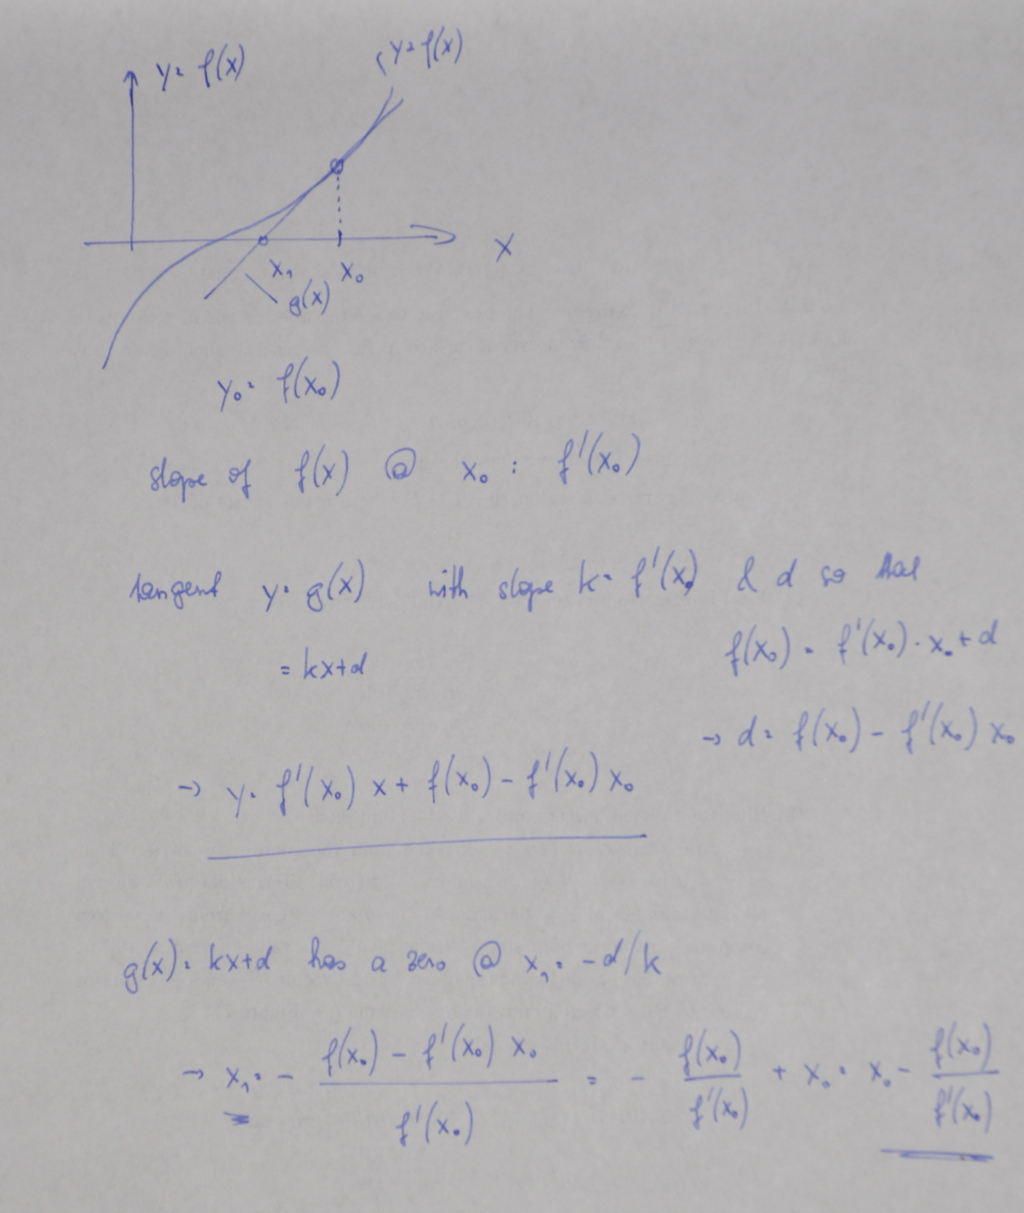
\includegraphics[scale=1.5]{images/DSC_0001_small.JPG}
\caption{Page1}
\end{figure}

e.g. \(f(x) = x^2-4\); then \(f'(x) = 2x\) and
\(x_{n+1} = x_n - (x^2-4)/(2x)\)

see
\href{file:///home/cnovak/src/julia/JuliaStuff/newton.jl}{newton.jl}:

\begin{verbatim}
function newton_solve(z0)
# solve x^2 - 4 = 0
    z = z0
    for n=1:20
        z = z - (z*2-4)/(2*z)
        println(n, " -> ", z)
    end
    return z
end

println(newton_solve(4))
\end{verbatim}

yields

\begin{verbatim}
1 -> 3.5
2 -> 3.0714285714285716
3 -> 2.722591362126246
4 -> 2.457185626921853
5 -> 2.271124947617549
6 -> 2.151745805619235
7 -> 2.0812236253398755
8 -> 2.0421967642419427
9 -> 2.021534326135688
10 -> 2.0108818599087837
11 -> 2.0054703734730377
12 -> 2.0027426475762127
13 -> 2.001373201741756
14 -> 2.000687071968178
15 -> 2.0003436539605324
16 -> 2.0001718564997053
17 -> 2.000085935632882
18 -> 2.000042969662595
19 -> 2.0000214852928857
20 -> 2.000010742761846
2.000010742761846
\end{verbatim}
